\PassOptionsToPackage{unicode}{hyperref}
\documentclass[aspectratio=1610, professionalfonts, 9pt]{beamer}

\usefonttheme[onlymath]{serif}
\usetheme[showtotalframes]{tudo}

\ifluatex
  \usepackage{polyglossia}
  \setmainlanguage{english}
\else
  \ifxetex
    \usepackage{polyglossia}
    \setmainlanguage{english}
  \else
    \usepackage[english]{babel}
  \fi
\fi

% Mathematik
\usepackage{amsmath}
\usepackage{amssymb}
\usepackage{mathtools}
\usepackage{cancel}

\usepackage{hyperref}
\usepackage{bookmark}
\usepackage{booktabs}       % stellt \toprule, \midrule, \bottomrule
\usepackage{graphicx}

%Einheiten
\usepackage[
  locale=DE,
  separate-uncertainty=true,
  per-mode=symbol-or-fraction,
  output-decimal-marker=.,
]{siunitx}
\sisetup{math-micro=\text{µ},text-micro=µ}

%%%%%%%%%%%%%%%%%%%%%%%%%%%%%%%%%%%%%%%%%%%%%%%%%%%%%%%%%%%%%%%%%%%%%%%%%%%%%%%%
%%%%%-------------Hier Titel/Autor/Grafik/Lehrstuhl eintragen--------------%%%%%
%%%%%%%%%%%%%%%%%%%%%%%%%%%%%%%%%%%%%%%%%%%%%%%%%%%%%%%%%%%%%%%%%%%%%%%%%%%%%%%%

%Titel:
\title{Decay kinematics comparison of pair-produced leptoquarks and vector-like quarks
in proton proton collisions at \(\sqrt{s}\) = 13 TeV at the LHC}
%Autor
\author[D.~Hellmann]{Dominik Hellmann}
%Lehrstuhl/Fakultät
\institute[E IV]{Experimentelle Physik 4 \\ Fakultät Physik}
%Titelgrafik
%\titlegraphic{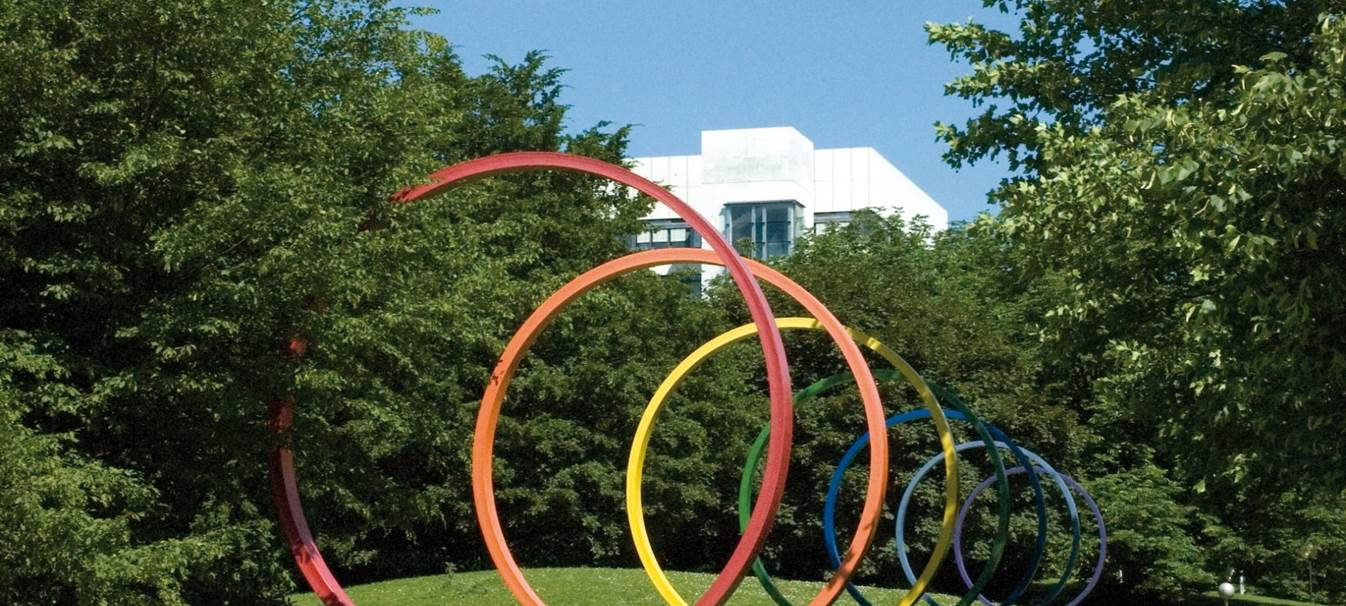
\includegraphics[width=0.7\textwidth]{images/tudo-title-2.jpg}}


\begin{document}

\maketitle
\begin{frame}{Table of Contents}
    \textbf{Introduction}
    \begin{itemize}
        \item leptoquark and vector-like quark properties
        \item considered decay modes
    \end{itemize}
    \textbf{Comparison of decay kinematics}
    \begin{itemize}
        \item existing vector-like quark analysis
        \item distributions of kinematic variables
    \end{itemize}
    \textbf{Top quark reconstruction}
    \begin{itemize}
        \item different reconstruction algorithms
        \item reconstruction and misreconstruction efficiencies
    \end{itemize}
    \textbf{New event selection}
    \begin{itemize}
        \item new event selection criteria
        \item efficiencies
    \end{itemize}
\end{frame}
%--------------------Einführung-------------------------------------------------
\section{Introduction}

\begin{frame}{leptoquarks and vector-like Quarks}
    \textbf{Motivation:}
    leptoquarks (LQ) could for example explain why there are the same number of generations of quarks and leptons,
    while vector-like quarks (VLQ) could solve the hierarchy problem of the SM
    \vspace{3mm}
    \begin{columns}[t]
        \begin{column}{0.5\textwidth}
            LQ:
            \begin{itemize}
                \item LQ multiplets are introduced by assuming conservation of \(B-L\)
                \item direct scalar or vector couplings to quarks and leptons \\
                \(\rightarrow\) Bosons: Spin 0 or 1 (model dependent)
            \end{itemize}
            Considered is the \(S_3\) LQ:
            \begin{itemize}
                \item assumed mass: \(m_{\mathrm{LQ}}=1000\,\mathrm{GeV}\)
                \item electric charge: \(Q=\frac{-1}{3}e\)
            \end{itemize}
        \end{column}
        \begin{column}{0.5\textwidth}
            VLQ:
            \begin{itemize}
                \item VLQs are introduced to modify Yukawa couplings of SM quarks
                \item Fermions: Spin 1/2
                \item transform like vectors under the electro-weak gauge group
            \end{itemize}
            Considered are \(B\) and \(T\) VLQ:
            \begin{itemize}
                \item assumed mass: \(m_{\mathrm{VLQ}}=1000\,\mathrm{GeV}\)
                \item electric charge: \(Q_{B}=\frac{-1}{3}e\) and \(Q_{T}=\frac{2}{3}e\)
                \item assumption: only coupling to 3rd generation quarks
            \end{itemize}
        \end{column}
    \end{columns}
\end{frame}

\begin{frame}{LQ and VLQ decays}
    \begin{columns}
        \begin{column}{0.5\textwidth}
            \begin{figure}
                \centering
                \includegraphics[width=0.975\textwidth]{img/LQ_feynman.pdf}
                \label{fig:LQ_fm}
            \end{figure}
            Feynman diagram of pair-produced LQ (\(\Phi\)) decays. \\
            Couplings are model dependent. \\
            Considered are cross generation decays: \(\Phi \rightarrow l^- t\) (\(l = e, \mu\))
        \end{column}
        \begin{column}{0.5\textwidth}
            \begin{figure}
                \centering
                \includegraphics[width=0.6\textwidth]{img/VLQ_W_feynman.pdf}
                \label{fig:VLQ_fm}
            \end{figure}
            Feynman diagram of pair-produced VLQ (\(B\)) decays.
            Couplings are model dependent. \\
            Other possible decay modes: \(B\mathrel{/}T \rightarrow Z (H) b\mathrel{/}t\)
        \end{column}
    \end{columns}
\end{frame}
%---------------------------------Comparison of decay kinematics----------------
\section{Comparison of decay kinematics}

\begin{frame}{VLQ reference event selection}
    \textbf{Preselection:}
    \begin{itemize}
        \item \(\ge 1\) opposite-sign same flavor (OS-SF) lepton pairs
        \item transverse momentum of OS-SF leptons: \(p_{\mathrm{T}} \ge 28 \, \mathrm{GeV}\)
    \end{itemize}
    \vspace{3mm}
    \textbf{Trilepton channel:}
    \begin{itemize}
        \item \(\ge 3\) leptons with \(p_{\mathrm{T}} \ge 28 \, \mathrm{GeV}\)
        \item at least 1 OS-SF lepton pair within a \(10 \, \mathrm{GeV}\) range of the Z boson mass
        \item \(\ge 1\) \(b\)-tagged jets
        \item transverse momentum of the same OS-SF lepton pair has to amount to \(\sum_{i=1}^{2} p_{\mathrm{T},i} \ge 200 \, \mathrm{GeV}\)
    \end{itemize}
    \vspace{3mm}
    \(\rightarrow\) this is an existing event selection of an ATLAS VLQ search (arXiv: 1806.10555 [hep-ex]) \\
    \(\rightarrow\) comparison of LQ and VLQ decay kinematics using \textbf{simulated truth level samples}
\end{frame}

\begin{frame}{Comparison of distributions of kinematic variables in LQ and VLQ processes}
    \textbf{lepton multiplicities are shown before (left) and after (right) the preselection:}\\
    \begin{columns}
        \begin{column}{0.5\textwidth}
            \begin{figure}
                \centering
                \includegraphics[width=\textwidth]{Histograms/lepton_multiplicity.pdf}
                \label{fig:lept_mult}
            \end{figure}
        \end{column}
        \begin{column}{0.5\textwidth}
            \begin{figure}
                \centering
                \includegraphics[width=\textwidth]{Histograms/lepton_multiplicity_pre.pdf}
                \label{fig:lept_mult_pre}
            \end{figure}
        \end{column}
    \end{columns}
    \(\rightarrow\) The requirement of 3 or more leptons is fulfilled by \(\approx 40 \. \%\) of all LQ events
\end{frame}

\begin{frame}{Comparison of distributions of kinematic variables in LQ and VLQ processes}
    \textbf{b quark multiplicity before (left) and after (right) the preselection:}\\
    \begin{columns}
        \begin{column}{0.5\textwidth}
            \begin{figure}
                \centering
                \includegraphics[width=\textwidth]{Histograms/b_multiplicity.pdf}
                \label{fig:b_mult}
            \end{figure}
        \end{column}
        \begin{column}{0.5\textwidth}
            \begin{figure}
                \centering
                \includegraphics[width=\textwidth]{Histograms/b_multiplicity_pre.pdf}
                \label{fig:b_mult_pre}
            \end{figure}
        \end{column}
    \end{columns}
    \(\rightarrow\) at least 2 b quarks occur in every LQ and VLQ event
\end{frame}

\begin{frame}{Comparison of distributions of kinematic variables in LQ and VLQ processes}
    \textbf{OS-SF pair transverse momentum distributions before and after the preselection:}
    \begin{columns}
        \begin{column}{0.5\textwidth}
            \begin{figure}
                \centering
                \includegraphics[width=\textwidth]{Histograms/Z_canditate_pt.pdf}
                \label{fig:ll_pt}
            \end{figure}
        \end{column}
        \begin{column}{0.5\textwidth}
            \begin{figure}
                \centering
                \includegraphics[width=\textwidth]{Histograms/Z_canditate_pt_pre.pdf}
                \label{fig:ll_pt_pre}
            \end{figure}
        \end{column}
    \end{columns}
    \(\rightarrow\) The largest amount of occuring LQ and VLQ events contain an OS-SF pair with \(p_{\mathrm{T}} > 200\,\)GeV
\end{frame}

\begin{frame}{Comparison of distributions of kinematic variables in LQ and VLQ processes}
    \textbf{OS-SF pair invariant mass distributions before (left) and after (right) the preselection:}
    \begin{columns}
        \begin{column}{0.5\textwidth}
            \begin{figure}
                \centering
                \includegraphics[width=\textwidth]{Histograms/next_to_m_Z_mass.pdf}
                \label{fig:ll_m}
            \end{figure}
        \end{column}
        \begin{column}{0.5\textwidth}
            \begin{figure}
                \centering
                \includegraphics[width=\textwidth]{Histograms/next_to_m_Z_mass_pre.pdf}
                \label{fig:ll_m_pre}
            \end{figure}
        \end{column}
    \end{columns}
    \(\rightarrow\) only a small amount of LQ events contain an OS-SF pair with an invariant mass with \(|m_{ll}-m_{Z}|<10\,\)GeV
\end{frame}


\begin{frame}{Reference selection --- cutflow}
  \textbf{event efficiencies after each cut in every sample but \(B\bar{B} \rightarrow HH b\bar{b}\):}
    \begin{figure}
        \centering
        \includegraphics[width=0.6\textwidth]{Histograms/trilepton_cutflow.pdf}
        \label{fig:triflow_old}
    \end{figure}
    \(\longrightarrow\) remaining LQ efficiency after all cuts: \(0.2_{-0.06}^{+0.09} \, \%\)
\end{frame}

\begin{frame}{Interim results}
    \textbf{Conclusions:}
    \begin{itemize}
        \item Z boson mass cut is too restrictive for LQ
        \item every other cut performs well for LQ due to similar decay topologies
    \end{itemize}
    \(\Rightarrow\) find a new criterion replacing the Z boson mass cut \\
    \vspace{3mm}
    This new cut has to be based on similar properties of LQ and VLQ. \\
    \(\rightarrow\) focus on top quarks from LQ and VLQ decays and develop a reconstruction algorithm \\
    \vspace{3mm}
    Divide top quark reconstruction according to its decay modes:
    \begin{itemize}
        \item hadronic: \(t \rightarrow W^{+} b \rightarrow q \bar{q}^{'} b \)
        \item leptonic: \(t \rightarrow W^{+} b \rightarrow l^{+} \nu_{l} b \)
    \end{itemize}
\end{frame}
%--------------------------Top quark reconstruction------------------------------
\section{Top quark reconstruction}

\begin{frame}{Hadronic reconstruction}
    Algorithm:
    \begin{itemize}
        \item collect all jet four-momentum information
        \item permute non b-tagged jets and find all combinations with \(|m_{W}-m_{q,q^{'}}| \le 5\,\mathrm{GeV}\)
        \item these \(W\) boson candidates are further permuted with \(b\)-tagged jets
        \item a top quark candidate is found if \(|m_{t}-m_{b,q,q^{'}}| \le 10\,\mathrm{GeV}\)
    \end{itemize}
\end{frame}

\begin{frame}{Hadronic reconstruction}
    Invariant masses of quark pairs originating from a W boson decay after a top quark decay (Left). \\
    Invariant masses of quark pairs and b quarks originating from a top quark decay (Right).
    \begin{columns}
        \begin{column}{0.5\textwidth}
            \begin{figure}
                \centering
                \includegraphics[width=\textwidth]{Histograms/invariant_mass_q_q_T.pdf}
                \label{fig:hadro_reco1}
            \end{figure}
        \end{column}
        \begin{column}{0.5\textwidth}
            \begin{figure}
                \centering
                \includegraphics[width=\textwidth]{Histograms/inv_mass_q_q_b_T.pdf}
                \label{fig:hadro_reco2}
            \end{figure}
        \end{column}
    \end{columns}
    \(\rightarrow\) the choice of reconstruction criteria is due to the sharp resonance peaks
\end{frame}

\begin{frame}{Leptonic reconstruction}
  For the leptonic reconstruction there are two cases:
  \begin{itemize}
    \item exactly one neutrino from a top quark decay \\
    \(\rightarrow\) top quark reconstruction from (\(l\),\(E_{\mathrm{T}}^\mathrm{{miss}}\),\(b\))
    \item \(> 1\) neutrino \(\rightarrow\) top quark reconstruction from (\(l\),\(b\))
  \end{itemize}
  \vspace{3mm}
  \begin{block}{\(E_{\mathrm{T}}^\mathrm{{miss}}\)}
    The \(E_{\mathrm{T}}^\mathrm{{miss}}\) vector contains the sum of all neutrino information accessible by a detector at the LHC.
    \begin{align*}
      p^{\mu}_{\mathrm{tot}}= \begin{pmatrix}E\\p_x\\p_y\\p_z\end{pmatrix} \quad \rightarrow \quad E_{\mathrm{T}}^\mathrm{{miss}} = \begin{pmatrix}E_{\mathrm{T}}\\p_x\\p_y\\0\end{pmatrix}
    \end{align*}
  \end{block}
\end{frame}

\begin{frame}{Leptonic reconstruction}
  \textbf{First case:}
  \begin{itemize}
    \item if a permutation (\(l\),\(E_{\mathrm{T}}^\mathrm{{miss}}\)) has an invariant mass with \(|m_{W}-m_{l,E_{\mathrm{T}}^\mathrm{{miss}}}| \le 15\,\mathrm{GeV}\) \\
    \(\rightarrow\) assign as \(W\) boson candidate
    \item if this \(W\) boson candidate and a \(b\) quark have an invariant mass with \(|m_{t}-m_{l,E_{\mathrm{T}}^\mathrm{{miss}},b}| \le 20\,\mathrm{GeV}\) \\
    \(\rightarrow\) a possible top quark candidate is found
    \item to reduce incorrect assignments: \(\Delta R_{b,l} < 1.5\)
  \end{itemize}
  \vspace{3mm}
  \textbf{Second case:}
  \begin{itemize}
    \item permute all \(b\) quarks and charged leptons
    \item if a permutation fullfills \(\Delta R < 1.5\) \\
    \(\rightarrow\) check if its invariant mass is within a \(50 \, \mathrm{GeV}\) range of \(105 \, \mathrm{GeV}\)
    \item then a top quark candidate is found
  \end{itemize}
\end{frame}

\begin{frame}{Leptonic reconstruction (first case)}
  invariant mass distributions of leptons and \(E_{\mathrm{T}}^\mathrm{{miss}}\) (left) and of b quarks,
  leptons and \(E_{\mathrm{T}}^\mathrm{{miss}}\) (right) originating from the same top quark decays:
    \begin{columns}
        \begin{column}{0.5\textwidth}
            \begin{figure}
                \centering
                \includegraphics[width=\textwidth]{Histograms/inv_mass_l_nu_T.pdf}
                \label{fig:lepto_reco1}
            \end{figure}
        \end{column}
        \begin{column}{0.5\textwidth}
            \begin{figure}
                \centering
                \includegraphics[width=\textwidth]{Histograms/inv_mass_b_l_nu_T.pdf}
                \label{fig:lepto_reco2}
            \end{figure}
        \end{column}
    \end{columns}
    \(\rightarrow\) the looser invariant mass criteria in the leptonic reconstruction are founded in the reduced neutrino momentum information
\end{frame}

\begin{frame}{Leptonic reconstruction (both cases)}
  \(\Delta R\) distributions of leptons and b quarks originating from the same (left) and from different (right) top quarks:
    \begin{columns}
        \begin{column}{0.5\textwidth}
            \begin{figure}
                \centering
                \includegraphics[width=\textwidth]{Histograms/Delta_R_b_t_l_T.pdf}
                \label{fig:lepto_reco3}
            \end{figure}
        \end{column}
        \begin{column}{0.5\textwidth}
            \begin{figure}
                \centering
                \includegraphics[width=\textwidth]{Histograms/Delta_R_b_t_l_T_bar.pdf}
                \label{fig:lepto_reco4}
            \end{figure}
        \end{column}
    \end{columns}
    \(\rightarrow\) most of the lepton and b quark pairs from the same top quark decay occur closer to each other resulting in a smaller value of \(\Delta R\) (<1.5)
\end{frame}

\begin{frame}{Leptonic reconstruction (second case)}
    invariant masses of b quarks and leptons from the same (left) and different (right) top quark decays:
    \begin{columns}
        \begin{column}{0.5\textwidth}
            \begin{figure}
                \centering
                \includegraphics[width=\textwidth]{Histograms/inv_mass_b_t_l_T.pdf}
                \label{fig:lepto_reco5}
            \end{figure}
        \end{column}
        \begin{column}{0.5\textwidth}
            \begin{figure}
                \centering
                \includegraphics[width=\textwidth]{Histograms/inv_mass_b_t_l_T_bar.pdf}
                \label{fig:lepto_reco6}
            \end{figure}
        \end{column}
    \end{columns}
    \(\rightarrow\) most of the lepton and b quark pairs from the same top quark decay have an invariant mass in a 50 GeV range around 105 GeV
\end{frame}

\begin{frame}{Reconstruction and misreconstruction efficiencies}
    \begin{columns}
        \begin{column}{0.5\textwidth}
            \begin{align*}
                R = \frac{\sum_{i = 1}^{N}\mathrm{tp}_i}{\sum_{i = 1}^{N}\mathrm{fn}_i + \mathrm{tp}_i} \\
                F = \frac{\sum_{i = 1}^{N}\mathrm{fp}_i}{\sum_{i = 1}^{N}\mathrm{tn}_i + \mathrm{fp}_i}
            \end{align*}
        \end{column}
        \begin{column}{0.5\textwidth}
            \begin{itemize}
                \item tp --- \# correctly reconstructed top quarks
                \item tn --- \# correctly discarded permutations
                \item fp --- \# falsely reconstructed top quarks
                \item fn --- \# falsely discarded permutations
            \end{itemize}
        \end{column}
    \end{columns}

    \begin{table}
        \centering
        \caption{Reconstruction and misreconstruction efficiencies for every reconstruction method across all samples. Uncertainties are calculated with the TEfficiency Root Class.}
        \label{tab:acc}
        \begin{tabular}{ccccc}
            \toprule
            {Sample} & {Leptonic \(R\mathrel{/}\si{\percent}\)} & {hadronic \(R\mathrel{/}\si{\percent}\)} & {Leptonic \(F\mathrel{/}\si{\percent}\)} & {hadronic \(F\mathrel{/}\si{\percent}\)}\\
            \midrule
            \(\Phi \bar{\Phi} \rightarrow l^+l^-t\bar{t}\) & \(69^{+1}_{-1}\) & \(93.03^{+0.31}_{-0.33}\) & \(4.23^{+0.14}_{-0.13}\) & \(1.11^{+0.06}_{-0.05}\)\\
            \(T\bar{T}\rightarrow ZZt\bar{t}\) & \(65.00^{+0.32}_{-0.32}\) & \(92.63^{+0.10}_{-0.10}\) & \(7.45^{+0.01}_{-0.01}\) & \(0.3259^{+0.0004}_{-0.0004}\)\\
            \(T\bar{T}\rightarrow HHt\bar{t}\) & \(53.91^{+0.32}_{-0.32}\)& \(92.75^{+0.10}_{-0.10}\) & \(4.31^{+0.06}_{-0.06}\) & \( 0.5089^{+0.0005}_{-0.0005}\)\\
            \(B\bar{B}\rightarrow W^+W^-t\bar{t}\) & \(58.0^{+0.5}_{-0.5}\) & \(92.69^{+0.14}_{-0.15}\) & \(13.94^{+0.13}_{-0.12}\) & \(1.927^{+0.001}_{-0.001}\)\\
            \bottomrule
        \end{tabular}
    \end{table}
\end{frame}

%-----------------------------New event selection--------------------------------
\section{New event selection}
\begin{frame}{Finding a new criterion}
    \textbf{New cut:} \\
    transverse momentum of reconstructed top quark candidates has to fulfill \(p_{\mathrm{T}} \ge 350 \, \mathrm{GeV}\) \\

    \begin{block}{Justification}
        This new criterion is based on the high top quark \(p_{\mathrm{T}}\) in considered event topologies \\
        \(\rightarrow\) the high LQ and VLQ mass is distributed equally on the energies of both of their decay products
    \end{block}
\end{frame}

\begin{frame}{Finding a new criterion}
  \textbf{transverse momentum distribution of actual (left) and reconstructed (right) top quarks:}
    \begin{columns}
        \begin{column}{0.5\textwidth}
            \begin{figure}
                \centering
                \includegraphics[width=\textwidth]{Histograms/top_pt.pdf}
                \label{fig:new_crit1}
            \end{figure}
        \end{column}
        \begin{column}{0.5\textwidth}
            \begin{figure}
                \centering
                \includegraphics[width=\textwidth]{Histograms/Top_reco_Pt.pdf}
                \label{fig:new_crit2}
            \end{figure}
        \end{column}
    \end{columns}
    \(\rightarrow\) the top quark reconstruction conserves the shape and position of the distributions
\end{frame}

\begin{frame}{Efficiencies}
  \begin{table}
      \caption{Event efficiencies after applying reference and new selection criteria with relative changes. Uncertainties are calculated with the TEfficiency Root Class.}
      \label{tab:final}
      \begin{tabular}{cccc}
          \toprule
          Sample & Efficiency of \(m_{Z}\) cut \(\mathrel{/}\si{\percent}\) & Efficiency of \(p_{\mathrm{T},t}\) cut \(\mathrel{/}\si{\percent}\) & Efficiency Ratio \\
          \midrule
          \(\Phi \bar{\Phi} \rightarrow l^+l^-t\bar{t}\)& \(0.20^{+0.09}_{-0.06}\) & \(23.9^{+0.6}_{-0.6}\) & \(118.40\)\\
          \(T\bar{T}\rightarrow ZZt\bar{t}\)& \(3.75^{+0.09}_{-0.09}\) & \(2.86^{+0.08}_{-0.07}\) & \(0.76\)\\
          \(B\bar{B}\rightarrow ZZb\bar{b}\)& \(0.492^{+0.033}_{-0.031}\) & \(0.040^{+0.011}_{-0.009}\) & \(0.10\)\\
          \(B\bar{B}\rightarrow W^+W^-t\bar{t}\)&  \(0.032^{+0.010}_{-0.008}\) & \(0.82^{+0.04}_{-0.04}\) & \(26.67\)\\
          \bottomrule
      \end{tabular}
  \end{table}
\end{frame}

\begin{frame}{Efficiencies}
  new event selection cutflow showing event efficiencies after applying each cut with the new top quark reconstruction criterion:
  \begin{figure}
    \centering
    \includegraphics[width=0.6\textwidth]{Histograms/triflow_new.pdf}
    \label{fig:newtriflow}
  \end{figure}
\end{frame}
%----------------------------Conclusions-----------------------------------------
\section{Conclusions}
\begin{frame}{Conclusions and Outlook}
  \textbf{Conclusions:}
  \begin{itemize}
    \item Z mass cut from the reference selection is too restrictive
    \item replacing it with a new cut based on top quark properties clearly improves efficiencies for LQ and VLQ samples
  \end{itemize}
  \(\Rightarrow\) A simultaneous search for LQ and VLQ seems to be possible \\
  \vspace{3mm}
  \textbf{Outlook:}
  \begin{itemize}
    \item the top quark reconstruction has to be further optimized \(\Rightarrow\) better efficiencies
    \item the event selection has to be tested on background samples to determine its sensitivity
  \end{itemize}
\end{frame}
%----------------------------------Danke-----------------------------------------
\section{}
\begin{frame}
    \Huge Thank you for your attention!!!
\end{frame}
%Nützliche Sachen
%--------------------Box auf Folie----------------------------------------------
%\begin{block}{title}
%\end{block}
%--------------------2 Zeilige Überschrift--------------------------------------
%Mit \frametitle{bla \newline bla2}
\end{document}
